%% BioMed_Central_Tex_Template_v1.06
%%                                      %
%  bmc_article.tex            ver: 1.06 %
%                                       %

%%IMPORTANT: do not delete the first line of this template
%%It must be present to enable the BMC Submission system to
%%recognise this template!!

%%%%%%%%%%%%%%%%%%%%%%%%%%%%%%%%%%%%%%%%%
%%                                     %%
%%  LaTeX template for BioMed Central  %%
%%     journal article submissions     %%
%%                                     %%
%%          <8 June 2012>              %%
%%                                     %%
%%                                     %%
%%%%%%%%%%%%%%%%%%%%%%%%%%%%%%%%%%%%%%%%%


%%%%%%%%%%%%%%%%%%%%%%%%%%%%%%%%%%%%%%%%%%%%%%%%%%%%%%%%%%%%%%%%%%%%%
%%                                                                 %%
%% For instructions on how to fill out this Tex template           %%
%% document please refer to Readme.html and the instructions for   %%
%% authors page on the biomed central website                      %%
%% http://www.biomedcentral.com/info/authors/                      %%
%%                                                                 %%
%% Please do not use \input{...} to include other tex files.       %%
%% Submit your LaTeX manuscript as one .tex document.              %%
%%                                                                 %%
%% All additional figures and files should be attached             %%
%% separately and not embedded in the \TeX\ document itself.       %%
%%                                                                 %%
%% BioMed Central currently use the MikTex distribution of         %%
%% TeX for Windows) of TeX and LaTeX.  This is available from      %%
%% http://www.miktex.org                                           %%
%%                                                                 %%
%%%%%%%%%%%%%%%%%%%%%%%%%%%%%%%%%%%%%%%%%%%%%%%%%%%%%%%%%%%%%%%%%%%%%

%%% additional documentclass options:
%  [doublespacing]
%  [linenumbers]   - put the line numbers on margins

%%% loading packages, author definitions

\documentclass[twocolumn]{bmcart}% uncomment this for twocolumn layout and comment line below
%\documentclass{bmcart}

%%% Load packages
\usepackage{amsthm,amsmath}
\usepackage{siunitx}
\usepackage{mfirstuc}
%\RequirePackage{natbib}
\usepackage[colorinlistoftodos]{todonotes}
\RequirePackage{hyperref}
\usepackage[utf8]{inputenc} %unicode support
%\usepackage[applemac]{inputenc} %applemac support if unicode package fails
%\usepackage[latin1]{inputenc} %UNIX support if unicode package fails
\usepackage[htt]{hyphenat}
\usepackage{array}

\newcolumntype{L}[1]{>{\raggedright\let\newline\\\arraybackslash\hspace{0pt}}p{#1}}

%%%%%%%%%%%%%%%%%%%%%%%%%%%%%%%%%%%%%%%%%%%%%%%%%
%%                                             %%
%%  If you wish to display your graphics for   %%
%%  your own use using includegraphic or       %%
%%  includegraphics, then comment out the      %%
%%  following two lines of code.               %%
%%  NB: These line *must* be included when     %%
%%  submitting to BMC.                         %%
%%  All figure files must be submitted as      %%
%%  separate graphics through the BMC          %%
%%  submission process, not included in the    %%
%%  submitted article.                         %%
%%                                             %%
%%%%%%%%%%%%%%%%%%%%%%%%%%%%%%%%%%%%%%%%%%%%%%%%%


%\def\includegraphic{}
%\def\includegraphics{}

%%% Put your definitions there:
\startlocaldefs
\endlocaldefs


%%% Begin ...
\begin{document}

%%% Start of article front matter
\begin{frontmatter}

\begin{fmbox}
\dochead{Report from 2015 Brainhack Americas (LA)}

%%%%%%%%%%%%%%%%%%%%%%%%%%%%%%%%%%%%%%%%%%%%%%
%%                                          %%
%% Enter the title of your article here     %%
%%                                          %%
%%%%%%%%%%%%%%%%%%%%%%%%%%%%%%%%%%%%%%%%%%%%%%

\title{Calculating the Laterality Index Using FSL for Stroke Neuroimaging Data}
\vskip2ex
\projectURL{Project URL: \url{http://github.com/npnl/LI\_FSL}}

\author[
addressref={aff1},
%
email={kaoriito@usc.edu}
]{\inits{KLI} \fnm{Kaori L.} \snm{Ito}}
\author[
addressref={aff1},
corref={aff1},
email={sliew@chan.usc.edu}
]{\inits{SLL} \fnm{Sook-Lei} \snm{Liew}}

%%%%%%%%%%%%%%%%%%%%%%%%%%%%%%%%%%%%%%%%%%%%%%
%%                                          %%
%% Enter the authors' addresses here        %%
%%                                          %%
%% Repeat \address commands as much as      %%
%% required.                                %%
%%                                          %%
%%%%%%%%%%%%%%%%%%%%%%%%%%%%%%%%%%%%%%%%%%%%%%

\address[id=aff1]{%
  \orgname{Neural Plasticity and Neurorehabilitation Laboratory, Chan Division of
Occupational Science and Occupational Therapy, Division of
Biokinesiology and Physical Therapy, Keck School of Medicine Department
of Neurology, University of Southern California},
  \city{Los Angeles},
  \street{1540 Alcazar Street, CHP 133 MC 9003},
  \postcode{90089},
  \postcode{California},
  \cny{USA}
}

%%%%%%%%%%%%%%%%%%%%%%%%%%%%%%%%%%%%%%%%%%%%%%
%%                                          %%
%% Enter short notes here                   %%
%%                                          %%
%% Short notes will be after addresses      %%
%% on first page.                           %%
%%                                          %%
%%%%%%%%%%%%%%%%%%%%%%%%%%%%%%%%%%%%%%%%%%%%%%

\begin{artnotes}
\end{artnotes}

%\end{fmbox}% comment this for two column layout

%%%%%%%%%%%%%%%%%%%%%%%%%%%%%%%%%%%%%%%%%%%%%%
%%                                          %%
%% The Abstract begins here                 %%
%%                                          %%
%% Please refer to the Instructions for     %%
%% authors on http://www.biomedcentral.com  %%
%% and include the section headings         %%
%% accordingly for your article type.       %%
%%                                          %%
%%%%%%%%%%%%%%%%%%%%%%%%%%%%%%%%%%%%%%%%%%%%%%

%\begin{abstractbox}

%\begin{abstract} % abstract
	
%Blank Abstract

%\end{abstract}



%%%%%%%%%%%%%%%%%%%%%%%%%%%%%%%%%%%%%%%%%%%%%%
%%                                          %%
%% The keywords begin here                  %%
%%                                          %%
%% Put each keyword in separate \kwd{}.     %%
%%                                          %%
%%%%%%%%%%%%%%%%%%%%%%%%%%%%%%%%%%%%%%%%%%%%%%

%\vskip1ex

%\projectURL{\url{http://github.com/npnl/LI\_FSL}}
%\projectURL{http://github.com/npnl/LI\_FSL}

% MSC classifications codes, if any
%\begin{keyword}[class=AMS]
%\kwd[Primary ]{}
%\kwd{}
%\kwd[; secondary ]{}
%\end{keyword}

%\end{abstractbox}
%
\end{fmbox}% uncomment this for twcolumn layout

\end{frontmatter}

%{\sffamily\bfseries\fontsize{10}{12}\selectfont Project URL: \url{http://github.com/npnl/LI\_FSL}}

%%% Import the body from pandoc formatted text
\section{Introduction}\label{introduction}

The laterality index (LI) is one way to assess hemispheric dominance in
a variety of tasks, such as language, cognitive functions, and changes
in laterality in clinical populations, such as after stroke. In stroke
neuroimaging, however, an optimal method of calculating the LI remains
controversial, largely due to lesion variability in post-stroke brains.

Two main methods of calculating LI have evolved in neuroimaging
literature \cite{Jansen2006}. The first, more traditional approach
counts the number of active voxels in a given region of interest (ROI)
for each hemisphere. This method has been criticized for its inability
to account for differences in signal intensity. Hence, a second approach
calculates laterality based on the percent signal change within a given
region; however, this method also has problems, such as difficulty
handling negative values.

A laterality toolbox that addresses some of these issues has been
implemented in the statistical neuroimaging analysis package SPM, which
provides users with options of using either method, along with more
advanced statistical tests for robust LI calculations \cite{Wilke2007}.
No such toolbox is yet available for FSL. Therefore, we developed a
series of scripts to calculate LI in FSL using both voxel count and
percent signal change methods. However, in the interest of space, here
we present only results from the more robust method of the two (voxel
count method).

\section{Approach}\label{approach}

We used fMRI data from two groups of stroke participants who either had
right or left hemisphere lesions. Participants observed videos of right
or left hand actions, and resulting statistical maps were calculated for
each individual. The LI was then calculated per participant, based on
the number of active voxels within a given anatomically-defined ROI (the
inferior frontal gyrus, pars opercularis). Using the ``cluster'' tool in
FSL, we set a threshold on the second-level whole-brain map. We set a
range of z-values (z=1.0, z=1.5, z=2.3) to test the effects of different
thresholds. We then utilized ``fslstats'' to determine the total number
of active voxels in both left and right hemisphere ROIs. Finally, we
calculated LI based on the equation:

\begin{verbatim}
LI=(L-R)/(L+R)
\end{verbatim}

where \emph{L} represents the number of active voxels in the
left-hemisphere ROI and \emph{R} is the number of active voxels in the
right-hemisphere ROI. This yields a value for LI such that -1
\textless{} \emph{LI} \textless{} +1, where a positive value indicates
left-hemisphere dominance and a negative value indicates
right-hemisphere dominance.

\begin{table*}[t!]
\caption{\label{stattable} Laterality Index Using a Voxel-Count-based Method in FSL: A Comparison Across Different Stroke Lesion Profiles and Different Thresholds}
\begin{tabular}{l l l l l l l l}
 \hline\noalign{\smallskip}
                         &            & \multicolumn{3}{c}{Subcortical Lesion} & \multicolumn{3}{c}{Cortical Lesion} \\
  Side of Stroke Lesion  & Z-score    & LH         & RH           & LI         & LH         & RH           & LI      \\
   \hline\noalign{\smallskip}
                         & 1          & 272        & 284          & -0.022     & 382        & 22           & 0.891 \\
  Left                   & 1.5        & 167        & 217          & -0.130     & 101        & 0            & 1  \\
                         & 2.3        & 37         & 123          & -0.538     & 1          & 0            & 1  \\         
 \hline  
 \emph{Mean}             &            &            &              & -0.230     &            &              & 0.964 \\
 \noalign{\smallskip}
                         & 1          & 335        & 68           &  0.662     & 509        & 49           & 0.824 \\
  Right                  & 1.5        & 193        & 29           &  0.739     & 318        & 3            & 0.981  \\
                         & 2.3        & 76         & 1            &  0.974     & 216        & 0            & 1  \\
  \hline
  \emph{Mean}            &            &            &              &  0.792     &            &              & 0.935 \\  
\end{tabular}
\end{table*}

\section{Results/Discussion}\label{resultsdiscussion}

We examined the variability in LI at different z-value thresholds to
look at laterality differences in individuals with cortical versus
subcortical stroke as well as the affected hemisphere (R vs.~L). The LI
values of four representative individuals (see Fig. \ref{fig1}) with the
following types of stroke were as follows (see Table 1): subcortical
left-hemisphere stroke (mean LI = -0.23; right lateralized), subcortical
right-hemisphere stroke (mean LI = 0.79; left lateralized), cortical
left-hemisphere stroke (mean LI = 0.96, left lateralized), and cortical
right-hemisphere stroke (mean LI = 0.94, left lateralized). These LI
results corresponded with our whole brain observations (not included
here), in which we examined the laterality of the action observation
network in individuals with left versus right hemisphere stroke (Ito,
OHBM 2016). Briefly, we show that most individuals show a
left-lateralized pattern of activity during action observation,
regardless of the lesion location. That is, Both individuals with
left-hemisphere stroke and individuals with right-hemisphere stroke tend
to activate the left, dominant hemisphere, suggesting a role of
hemispheric dominance during recovery after stroke.

\begin{figure}[h!]
  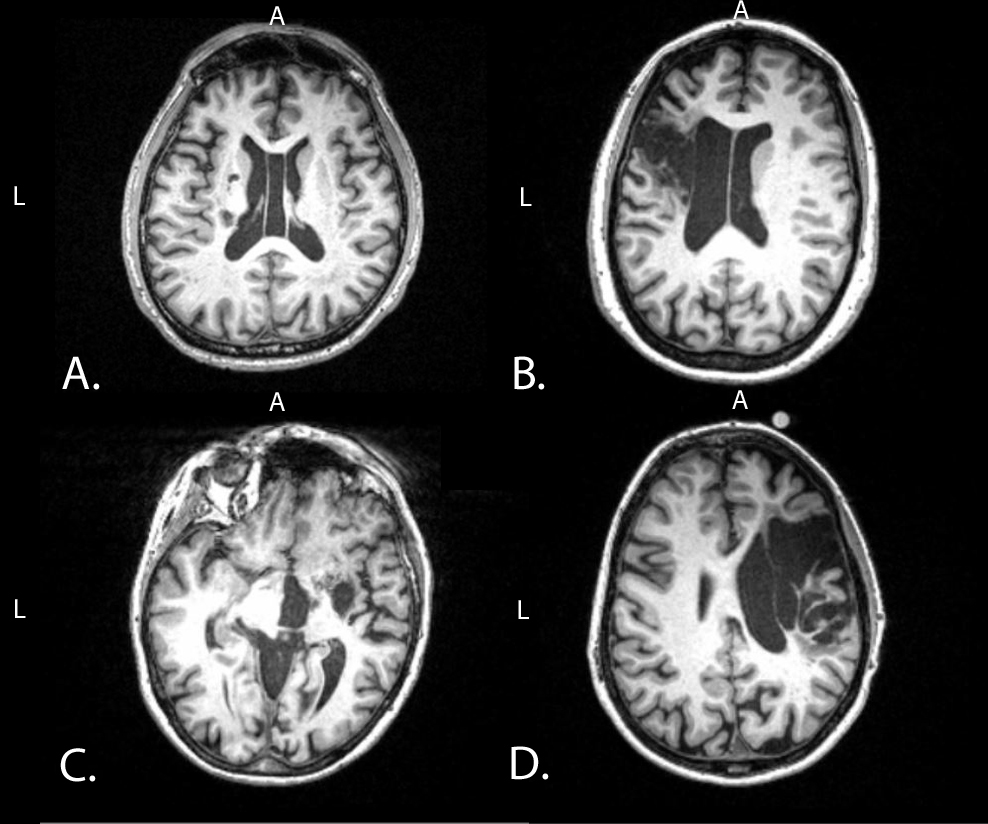
\includegraphics[width=.47\textwidth]{desmxz.jpg}
  \caption{\label{fig1}
  A Comparison Across Different Stroke Lesion Profiles at Maximum Lesion. MRI scans of individuals who sustained A. subcortical left-hemisphere stroke, B. cortical left-hemisphere stroke, C. subcortical right-hemisphere stroke, D. cortical right-hemisphere stroke. }
\end{figure}

\begin{figure}[h!]
  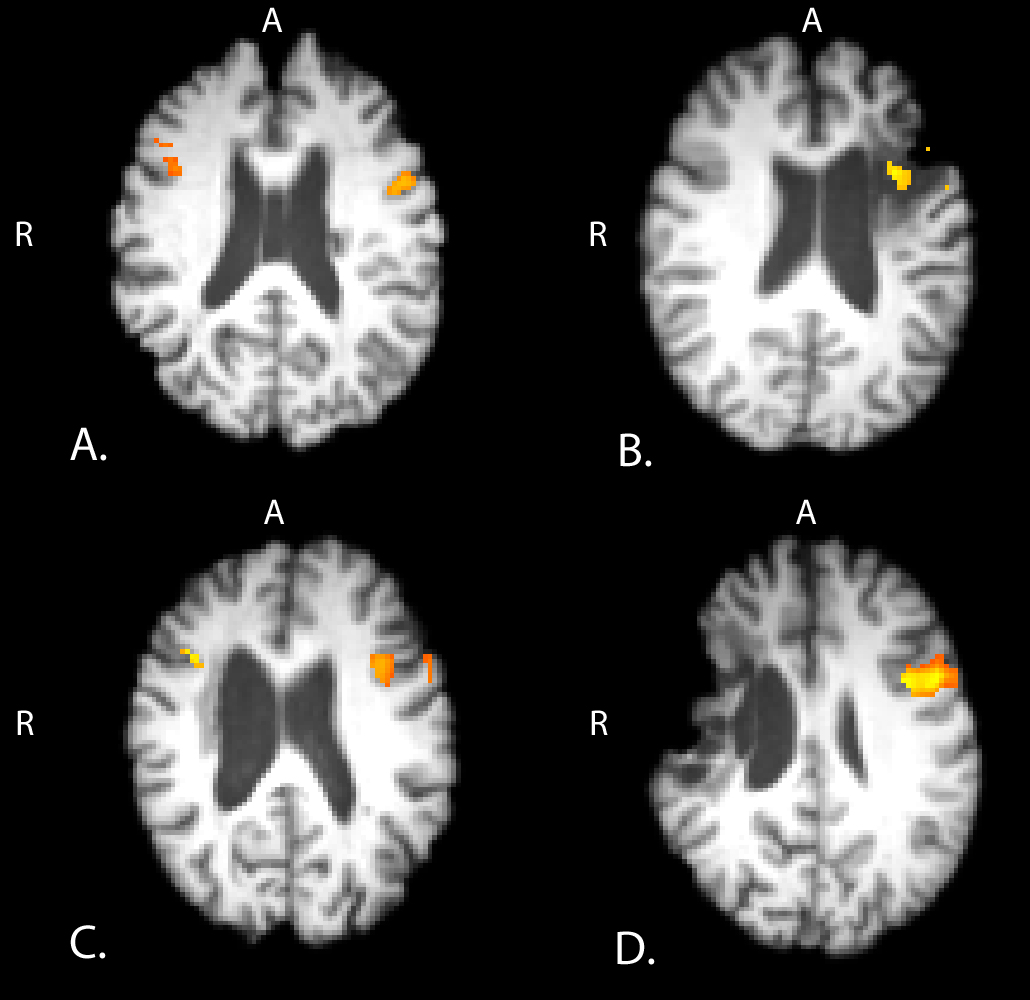
\includegraphics[width=.47\textwidth]{activation_standardSpace.jpg}
  \caption{\label{fig2}
  Overlap Between Activation in ROI and Lesion. Activity in the inferior frontal gyrus, pars opercularis at z=1.5 for individuals who sustained A. subcortical left-hemisphere stroke, B. cortical left-hemisphere stroke, C. subcortical right-hemisphere stroke, D. cortical right-hemisphere stroke. Images were registered to standard space. }
\end{figure}

Importantly, we notice that the voxel count method is highly dependent
on the threshold value: as the threshold increases in stringency, the
value of the LI increases. With individuals after stroke, higher
thresholds may yield 0 active voxels, leading to a potentially skewed LI
(LI=1).

\section{Conclusions}\label{conclusions}

We suggest that stroke neuroimaging might benefit from calculating an
average LI across different thresholds (including more lenient
thresholds such as z=1.0), in order to provide a more robust outcome
that takes into account threshold dependency. This is especially true
for individuals with cortical strokes, where the ROI may overlap with
the lesion and yield 0 active voxels. This issue of thresholding,
specifically for stroke research, is an interesting question that
remains to be addressed further. Future work may also utilize
threshold-weighted overlap maps to visualize subject variablility when
using different thresholds to calculate a laterality index
\cite{Seghier2016}. Our scripts for these calculations may be found
online at \url{http://chan.usc.edu/npnl/resources}.

%%%%%%%%%%%%%%%%%%%%%%%%%%%%%%%%%%%%%%%%%%%%%%
%%                                          %%
%% Backmatter begins here                   %%
%%                                          %%
%%%%%%%%%%%%%%%%%%%%%%%%%%%%%%%%%%%%%%%%%%%%%%

\begin{backmatter}

\section*{Availability of Supporting Data}
More information about this project can be found at: \url{http://github.com/npnl/LI\_FSL}. Further data and files supporting this project are hosted in the \emph{GigaScience} repository REFXXX.

\section*{Competing interests}
None

\section*{Author's contributions}
KLI and SLL wrote the software, performed tests, and wrote the report.

\section*{Acknowledgements}
The authors would like to thank the organizers and attendees of
Brainhack LA and the developers of FSL. This project was funded in part
by a Educational Research Grant from Amazon Web Services.

  
  
%%%%%%%%%%%%%%%%%%%%%%%%%%%%%%%%%%%%%%%%%%%%%%%%%%%%%%%%%%%%%
%%                  The Bibliography                       %%
%%                                                         %%
%%  Bmc_mathpys.bst  will be used to                       %%
%%  create a .BBL file for submission.                     %%
%%  After submission of the .TEX file,                     %%
%%  you will be prompted to submit your .BBL file.         %%
%%                                                         %%
%%                                                         %%
%%  Note that the displayed Bibliography will not          %%
%%  necessarily be rendered by Latex exactly as specified  %%
%%  in the online Instructions for Authors.                %%
%%                                                         %%
%%%%%%%%%%%%%%%%%%%%%%%%%%%%%%%%%%%%%%%%%%%%%%%%%%%%%%%%%%%%%

% if your bibliography is in bibtex format, use those commands:
\bibliographystyle{bmc-mathphys} % Style BST file
\bibliography{brainhack-report} % Bibliography file (usually '*.bib' )

\end{backmatter}
\end{document}
